\documentclass[numbers=noenddot, 12pt, a4paper, oneside]{scrbook}
\usepackage{blindtext}
\usepackage[utf8]{inputenc}
\usepackage{float}
\usepackage{tabularx}
\usepackage{graphicx}
\def\Plus{\texttt{+}}
\usepackage[final]{pdfpages}
\usepackage[procnames]{listings}
\usepackage{color}
\definecolor{lightgray}{rgb}{.9,.9,.9}
\definecolor{darkgray}{rgb}{.4,.4,.4}
\definecolor{purple}{rgb}{0.65, 0.12, 0.82}



\lstdefinelanguage{JavaScript}{
	keywords={typeof, new, true, false, catch, function, return, null, catch, switch, var, if, in, while, do, else, case, break},
	keywordstyle=\color{blue}\bfseries,
	ndkeywords={class, export, boolean, throw, implements, import, this},
	ndkeywordstyle=\color{darkgray}\bfseries,
	identifierstyle=\color{black},
	sensitive=false,
	comment=[l]{//},
	morecomment=[s]{/*}{*/},
	commentstyle=\color{purple}\ttfamily,
	stringstyle=\color{red}\ttfamily,
	morestring=[b]',
	morestring=[b]"
}

\lstset{
	language=JavaScript,
	backgroundcolor=\color{lightgray},
	extendedchars=true,
	basicstyle=\footnotesize\ttfamily,
	showstringspaces=false,
	showspaces=false,
	numbers=left,
	numberstyle=\footnotesize,
	numbersep=9pt,
	tabsize=2,
	breaklines=true,
	showtabs=false,
	captionpos=b
}

\lstset{frame=tb,
	language=Java,
	aboveskip=3mm,
	belowskip=3mm,
	showstringspaces=false,
	columns=flexible,
	basicstyle={\small\ttfamily},
	numbers=none,
	numberstyle=\tiny\color{gray},
	keywordstyle=\color{blue},
	commentstyle=\color{dkgreen},
	stringstyle=\color{red},
	breaklines=true,
	breakatwhitespace=true,
	tabsize=3
}

\definecolor{keywords}{RGB}{255,0,90}
\definecolor{comments}{RGB}{0,0,113}
\definecolor{red}{RGB}{160,0,0}
\definecolor{green}{RGB}{0,150,0}

\lstset{language=Python, 
	basicstyle=\ttfamily\small, 
	keywordstyle=\color{keywords},
	commentstyle=\color{comments},
	stringstyle=\color{red},
	showstringspaces=false,
	identifierstyle=\color{green},
	procnamekeys={def,class}}


\begin{document}

 
\begin{titlepage}
	\centering
	{\scshape\LARGE Politecnico di Milano \par}
	\vspace{1cm}
	
\includegraphics[width=0.65\textwidth]{polimi-logo}\par
	\vspace{1cm}
		
	{\scshape\Large Software Engineering 2 Course\par}
	\vspace{1.5cm}
	{\huge\bfseries Travlendar \Plus \par}
	\vspace{1cm}
	{\Large\bfseries Implemetation \& Testing Document \par}
	\vspace{3cm}
	{\Large\itshape di\par}
	{\Large\itshape Gianluigi Oliva, Marco Mussi e Lukasz Moskwa\par}
	\vspace{1.5cm}
	Github: https://github.com/Gigioliva/OlivaMussiMoskwa\\
	Heroku: http://travlendarmom.herokuapp.com/
	\vfill

	
	\vfill
	
	% Bottom of the page
	{\large \today\par}
\end{titlepage}

\newpage 
\tableofcontents
\newpage 

\chapter{Introduction and Scope}
Travlendar+ allows to create a calendar which fits the meetings and other kind of commitments. The key feature of this application is to determine if the meeting location is reachable in the scheduled time and then provide a fast way to get to the destionation, otherwise it notify the user that it is not possibile by any mean to fullfill the request. Furthermore the application also arranges the schedule in a flexible way for some kind of events (like the lunch) and offers the possibility to slightly change its time.\\
In the creation of the user's calendar it also takes into account the current weather condition to make smarter decisions. As example, if the user show interest in using bike or a bike sharing service, during a sunny day, the system will favor a suitable path.\\\newline

This document have the scope o present all things implemented related to that described in the RASD and DD and will be underlined the functionalities and the requirements that are and aren't implemented with the related motivations. \\\newline

In the following pages will be described the procedure that permit to install and start the whole platform showing all the external software and configuration files required to execute the system properly.
Furthermore in order to easy the usage will be provided an URL through which is possible to use the platform without installing any software. \\\newline
With the purpose to validate both the server side both the client side they will be written some tests with the aim to verify the correctness of the execution using dedicated tools. \\\newpage


\chapter{Requirements and Functionalities}

In this chapter we will talk about the Functional Requirements that were implemented and those that were not with a motivation for each one.\\

In particular we implemented the following functionalities:
\begin{itemize}
	\item Register to Travlendar+
	\item Create a daily schedule
	\item Manage user's own data
	\item Retrieve information about the weather forecast
	\item Modify an already completed schedule for a certain day
	\item Modify user's preferred time for having a meal
	\item Receive information about the current journey
\end{itemize}

These were implemented in order to provide all the basic functionalities that allow an effective use of the platform.\\\newline

On the other hand, we could not implement the following functionalities:
\begin{itemize}
	\item Buy tickets and subscriptions
	\begin{itemize}
		\item We have no access to the API of the ATM and Trenord for the purchase of tickets and subscriptions
	\end{itemize}
	\item Reservation of car and mobile sharing services
	\begin{itemize}
		\item We have no access to the API of the shared means of transport (like Enjoy, Mobike, OFO ect)
	\end{itemize}
\end{itemize}


\chapter{Frameworks}

As explained prevously in the DD, while realizing the application we used the follwing programming and markup languages and frameworks:

\section*{Programming Languages}

For the \underline{server side} we used the following programming languages:
\begin{itemize}
	\item \textbf{Java 8}
	\begin{itemize}
		\item We decided to use Java 8 to deply the main server of our application\\
		\textbf{PRO}: Ease the collaboration one the same code and it is portable. It also has a huge number of available libraries free to use\\ 
		\textbf{CON}: It's slow
	\end{itemize}
	\item \textbf{Python}
	\begin{itemize}
		\item We used python to develop a server with the only purpose to validate the interaction between the client and server side.\\
		\textbf{PRO}: Reliable and allows a fast implementation of the software required.\\
		\textbf{CON}: No perceivable cons
	\end{itemize}
	\item \textbf{SQL}
	\begin{itemize}
		\item We used SQL for the management of data\\
		\textbf{PRO}: It supports relational databases and work on all the main DBMS\\
	\end{itemize}
\end{itemize}



For the \underline{client side} we used the following programming and markdown languages:
\begin{itemize}
	\item \textbf{HTML 5}
	\begin{itemize}
		\item Last version of the common used language to develop web sites\\
		\textbf{PRO}: Easy to use, supported by all the browsers\\
	\end{itemize}
	\item \textbf{CSS 3}
	\begin{itemize}
		\item Last version of the common used language to edit style of web pages\\
		\textbf{PRO}: Really awesome effects\\
		\textbf{CON}: Lack of variables easy to use\\
	\end{itemize}
	\item \textbf{JavaScript}
	\begin{itemize}
		\item Common used language to perform dynamic actions on web pages\\
		\textbf{PRO}: Lot of libraries and not so hard to implement\\
		\textbf{CON}: There is no debugging in easy way. Sometimes workarounds are required in order to make an acceptable code
		\\
	\end{itemize}
\end{itemize}


\section*{Framework}

For the server side we used the following libraries and frameworks:
\begin{itemize}
	\item \textbf{Java}:
	\begin{itemize}
		\item JavaEE
		\item JUnit
		\item org.json
		\item google.gson
		\item org.PostgreSQL
		\item PowerMockito
		\item Mockito
	\end{itemize}
	\item \textbf{Python}:
	\begin{itemize}
		\item colorama
		\item Flask
		\item json
		\item pprint
	\end{itemize}
\end{itemize}

For the client side we used the following libraries and frameworks:
\begin{itemize}
	\item \textbf{Template}: REGNA Template (Free Version)
	\item \textbf{Phonegap} and Cordova for cross-compiling
	\item \textbf{Javascript} Libraries:
	\begin{itemize}
		\item fullcalendar.js (from fullcalendar.io)
		\item jQuery
		\item Bootstrap
		\item maps.googleapis.com
		\item Moment
	\end{itemize}	
\end{itemize}

\section*{Other software used}

\begin{itemize}
	\item Tomcat
	\item MySQL
	\item Postgress
	\item Flask
	\item Apache JMeter
	\item Heroku
\end{itemize}

The last one was used to deploy the application server to a remote host. Due to this, in order to use the platform, is enough to connect to a URL provided in the respective section of installation. 

\section*{Used API}

\begin{itemize}
	\item \textbf{Google API}: These are used to display and receive information about the path and everything concerning the journey.
	
	\item \textbf{APIXU API}: These are use in order to receive and display the data about the weather forecast in a particular day.
	
	\item \textbf{IMGUR API} These are use in order to save the picture of the user.
\end{itemize}



\chapter{Structure of the code}


As often said in the other documents, the system was parted in three layers: presentation, application and data layer. Each of these levels is executed on a separate machine/server in order to guarantee a three-tier architecture, as explained in the DD, increasing the overall security.\\

\section*{Server Side}
\lstset{language=Java}
The Data layer is built with tables that are populated with the information of all the users and implemented with SQL language.\\
On the other hand, the Application layer contains all the business logic and functions and it was implemented in Java. That also allowed a logical partition of different modules:
\begin{itemize}
	\item \textbf{DataHandlerDBMS}: This module takes care of the connection and communication with the DBMS, enabling the possibility of receiving query and DML commands.
	\item \textbf{UserManager}: This module handles all the data of a single user and functions like Login, Logout and information update. For the login and logout it also take advantage of the SecurityAuthenticator for handling the token that identifies the user.
	\item \textbf{ScheduleManager}: This module takes care of the user's schedule management by enabling the function of creating a new one, making sure it does not already exist, populate it with events of any kind, making sure there are no overlaps and using the best route for a journey. For the selection of the path we make use of ExternalRequestManager class which interfaces with an external API to get information about the route and the weather.
	\item \textbf{Servlet}: This module is responsible for the communication of the application layer with the presentation one by defining the endpoints on which the GET and POST will work, handling requests and returning the result of the application server for the requested function.
	\item \textbf{Data}: This module contains all the classes that represent the data stored in the DB in order to facilitate their use when required. Also within them, there are the methods that transform those data in JSON and then send them to various clients.
\end{itemize}

% Esempio di codice da inserire per Java

\textbf{Example of code for database request}:
\begin{lstlisting}
	public static ResultSet sendQuery(String query) {
		try {
				Statement stm = DBMS.createStatement();
				ResultSet res = stm.executeQuery(query);
				return res;
		} catch (SQLException e) {
				System.out.println("Error in sendQuery");
				e.printStackTrace();
		}
		return null;
	}
\end{lstlisting}

\textbf{Example of code for addEvent}:
\begin{lstlisting}
public static boolean addEvent(User user, String day, Event event, String origin) {
	String username = user.getUsername();
	ArrayList < TypeMeans > means = user.getMeansPref();
	Schedule schedule = getSchedule(username, day);
	Time t = null;
	TypeMeans meansUsed = null;
	int wheater = ExternalRequestManager.getWeatherForecast(origin, day);
	for (TypeMeans el: means) {
		HashMap < String, Integer > ris = ExternalRequestManager.getDistanceMatrixAPI(origin, event.getPosition(),
		el.getTypeAPI());
		if (ris != null) {
				Time temp = new Time((ris.get("duration") - 3600) * 1000);
					if (el == TypeMeans.bicycling && wheater == 1000) {
						if (t == null || temp.compareTo(t) < 0) {
							t = temp;
							meansUsed = el;
						}
					}
				if (el == TypeMeans.walking && ris.get("distance") <= user.getMaxWalk()) {
					if (t == null || temp.compareTo(t) < 0) {
						t = temp;
						meansUsed = el;
					}
				}
				if (el == TypeMeans.driving) {
					if (t == null || temp.compareTo(t) < 0) {
						t = temp;
						meansUsed = el;
					}
				}
				if (el.isTransit() && user.getMaxHoursMeans().compareTo(event.getStart()) >= 0) {
					if (t == null || temp.compareTo(t) < 0) {
						t = temp;
						meansUsed = el;
					}
				}
			}
		}
		if (t != null && meansUsed != null) {
			int startJourney = (int)(event.getStart().getTime() - t.getTime() - 3600000);
			if (startJourney < -3600000) {
				return false;
			}
			Journey j = new Journey(new Time(event.getStart().getTime() - t.getTime() - 3600000), t, meansUsed, event, origin);
			boolean notOverlaps = true;
			ArrayList < Journey > breakEx = schedule.getAndRemoveBreak();
			Time startj = j.getStart();
			Time endj = new Time(event.getStart().getTime() + event.getDuration().getTime() + 3600000);
			for (Journey el: schedule.getSchedule()) {
				Time startEl = el.getStart();
				Time endEl = new Time(
				el.getEvent().getStart().getTime() + el.getEvent().getStart().getTime() + 3600000);
				if ((startj.compareTo(startEl) > 0 && startj.compareTo(endEl) < 0) || (endj.compareTo(startEl) > 0 && endj.compareTo(endEl) < 0)) {
					notOverlaps = false;
					break;
				}
			}
			if (notOverlaps && canAddBreak(user, schedule)) {
				for (Journey el: breakEx) {
					deleteEvent(el.getEvent().getID());
				}
			DataHandlerDBMS.executeDML("insert into event (ID, name, start, duration, type, position) values (" + event.stringValuesQuery() + ")");
			DataHandlerDBMS.executeDML( "insert into journey (username, day, start, duration, path, EventID, position) values ('" + username + "','" + day + "'," + j.stringValuesQuery() + ")");
			for (Journey el: breakEx) {
				Break br = user.getBreakFromName(el.getEvent().getName());
				if (br != null) {
					addBreak(br, user, day);
				}
			}
			return true;
			} else {
				return false;
			}
		} else {
			return false;
		}
}
\end{lstlisting}

\section*{Client Side}

The Presentation Layer instead is written mainly with Web based laguages like HTML5, CSS3 and JavaScript. Then, in order to obtain a mobile version executable, the Web Application is parsed and compiled with Phonegap. \\

The website is parted as follows in order to cover all the functions required:
\begin{itemize}
	\item \textbf{index.html}: This is the intial page with a welcome screen and a brief description of the application. From this page is actually possibile to perform a Sign Up action to register a new user or a Sign In action to login with an existing user.
	\item \textbf{main.html}: This is the main page where a calendar with all the schedules can be seen. It is also possibile to change the basic view of the calendar from day to month and create a new Schedule for a chosen day. Then, the user can also create a new Event filling a brief form. 
	\item \textbf{profile.html}: In this page the user can actually see all the information about his/her profile and update them: it is possible to set a preferred range for a break during a day with a schedule, adding/removing means of transport from the preferred ones and change personal information like credit card number, driving license number and update the profile picture.
	\item \textbf{weather.html}: In this page a user can actually check the weather for a chosen day
	\item \textbf{ticket.html}: This page was realized only for the sake of completeness. As we can't realize a concrete communication with third part API for the purchase of tickets and subscription, there is only a layout left for future implementations.
\end{itemize}

About the code structure, the business logic of the client was completely implemented with JavaScript and some of its libraries. Some examples are provided as follows:\\ 

\lstset{language=JavaScript}
\textbf{Example of code for basic client-server request}:

\begin{lstlisting}
	var isPhoneGap = true; //changed on server side to false, true for mobile
	var herokuURL = "";
	if (isPhoneGap) {
		herokuURL = "http://travlendarmom.herokuapp.com";
	}


	$.ajax({
		dataType: "text",
		contentType: "text/plain; charset=utf-8",
		type: "POST",
		url: herokuURL + "/ExampleEndpoint",
		data: JSON.stringify(dataToSend),
		success: function(response) {
			//Function to execute in case of success
		}
	});
\end{lstlisting}

This type of request is often performed in order to receive information from the server side. The response is then analyzed and parsed in order to show data to the user on the client side.\\

\textbf{Working code for retrieving data and create a calendar}:

\begin{lstlisting}
	$('#calendar').fullCalendar({
		header: {
			left: 'title',
			right: 'prev,next today month agendaDay'
		},
		dayClick: function(date, jsEvent, view, resourceObj) {
			$('#calendar').fullCalendar("gotoDate", date);
			$('#calendar').fullCalendar('changeView', 'agendaDay');
		},
		views: {
			listDay: {
				buttonText: 'Day'
			},
			listWeek: {
				buttonText: 'Week'
			}
		},
		eventClick: function(calEvent, jsEvent, view) {
		
			var moment = $('#calendar').fullCalendar('getDate');
			var time_no = String(moment.format()).split("T")[0].split("-");
			var time_send = time_no[2] + "-" + time_no[1] + "-" + time_no[0];
			var coseDaMandare = {
				"username": localStorage.getItem("my_username"),
				"token": localStorage.getItem("my_travlendar"),
				"day": time_send
			};
			$.ajax({
				dataType: "text",
				contentType: "text/plain; charset=utf-8",
				type: "POST",
				url: herokuURL + "/GetSchedule",
				data: JSON.stringify(coseDaMandare),
				success: function(response) {
					response = JSON.parse(response);
					var scorrimento = response["schedule"]["singleSchedule"];
					for (var i = 0; i < scorrimento.length; i++) {
						if (scorrimento[i]["event"]["ID"] == calEvent.id) {
							var coseDaMandare = {
								"origin": scorrimento[i]["position"],
								"destination": scorrimento[i]["event"]["position"],
								"mode": scorrimento[i]["means"]
							};
							$.ajax({
								dataType: "text",
								contentType: "text/plain; charset=utf-8",
								type: "POST",
								url: herokuURL + "/GetPath",
								data: JSON.stringify(coseDaMandare),
								success: function(response) {
									console.log(response);
								}
							});
						}
					}
				}
			});
		},
		defaultView: 'agendaDay',
		navLinks: true, 
		editable: false,
		eventLimit: true,
		events: returnArray, 
		eventColor: '#212170',
		eventTextColor: "white",
		eventBorderColor: "blue"
	});
\end{lstlisting}

As it's possible to see by the code, in order to view the calendar the user is required to have an access token provided by the application server, then he need to previously login.


\chapter{Testing}

In order to proof the correctness of the most important parts of the code will be provided a complete test of all the main client and server parts of the code.

\section*{Server Testing}
On server side the Java EE code has been tested using the tools that Java provide with some additional libraries. In particular were used the JUnit libraries to test the part that works completely in the local system without using external resources like DBMS and network.
To emulate the part which requires the interaction with external component was used a framework called Mockito to test all the part that regards the not static classes and methods of the code and another derivative tool called PowerMockito to emulate the execution and the response of the parts of the code which are the static. 
The test of the Java EE server is available with the source code of the whole Web Application in Travlendar/src/test folder in the Github repository.
The server test is repetible by Right Click on src folder in Eclipse $\,\to\,$ Run as $\,\to\,$ JUnit test.\\

Furthermore in order to measure the performance of the whole server side will be showed in the next pages some reports of the performance measurerement made by Apache JMeter.
All tests are executed using Apache JMeter version 3.3 (JMeter can be downloaded from \textbf{http://jmeter.apache.org/}).

In order to make the performance measurement test repeatable easily the target of the test provided in the folder TestExtra/testJMeter folder in the Github repository have as target the Heroku site.
The performance tests must be executed in this order:
\begin{itemize}
	\item First must be executed the login method with the parameters like in the Login.jmx file (username:admin and password:pass)
	\item After the execution of the login performance test in the response section a token will be retuned
	\item Returned token must be inserted in the proper space in "Body Data" field (HTTP Request section) of the others performace tests in order to authenticate the user properly on the system, otherwise the user result ont properly logged in
\end{itemize}

All the results of the tested method are showed in the next pages.
\begin{figure}[H]
	\centering
	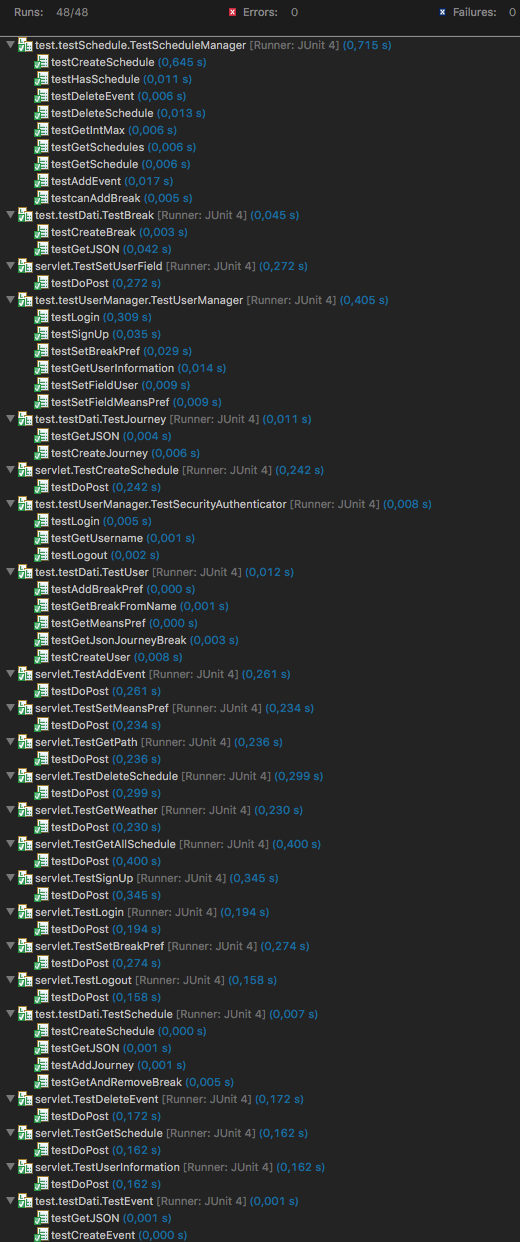
\includegraphics[width=0.5\textwidth]{Test/ServerEclipse}
	\caption{The result of the JUnit test on Eclipse}
\end{figure}

\begin{figure}[H]
	\centering
	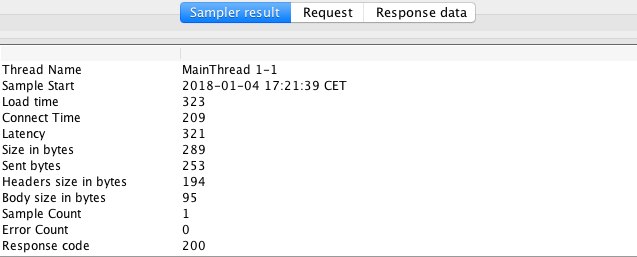
\includegraphics[width=0.9\textwidth]{Test/LoginMain}
	\caption{The performance results (in millisecond) of the Login servlet on Heroku application server}
\end{figure}

\begin{figure}[H]
\centering
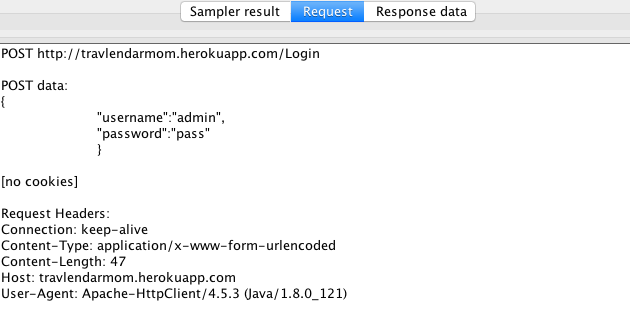
\includegraphics[width=0.8\textwidth]{Test/LoginReq}
\caption{The request sended to server for the Login servlet}
\end{figure}

\begin{figure}[H]
\centering
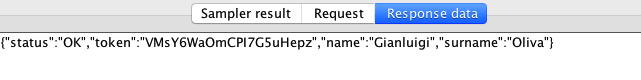
\includegraphics[width=0.8\textwidth]{Test/LoginResp}
\caption{The response of the server for the Login servlet}
\end{figure}

\begin{figure}[H]
	\centering
	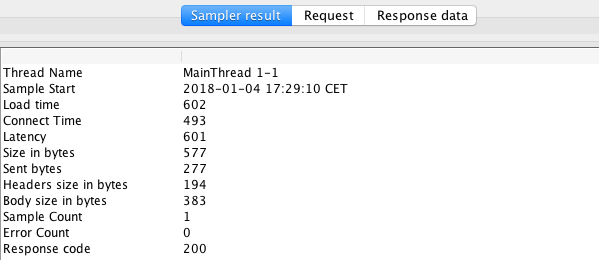
\includegraphics[width=0.8\textwidth]{Test/UserInformationMain}
	\caption{The performance results (in millisecond) of the UserInformation servlet on Heroku application server}
\end{figure}

\begin{figure}[H]
	\centering
	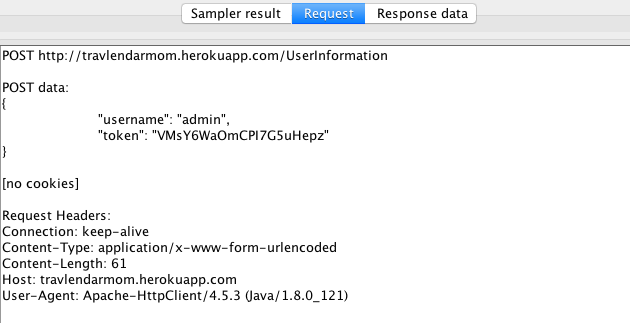
\includegraphics[width=0.8\textwidth]{Test/UserInformationReq}
	\caption{The request sended to server for the UserInformation servlet}
\end{figure}

\begin{figure}[H]
	\centering
	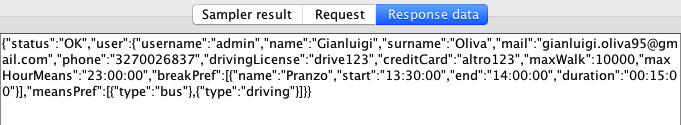
\includegraphics[width=0.8\textwidth]{Test/UserInformationResp}
	\caption{The response of the server for the UserInformation servlet}
\end{figure}

\begin{figure}[H]
	\centering
	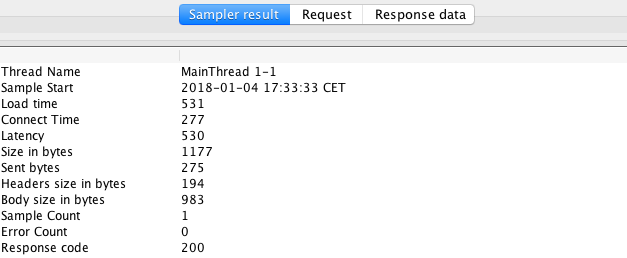
\includegraphics[width=0.8\textwidth]{Test/GetAllScheduleMain}
	\caption{The performance results (in millisecond) of the GetAllSchedule servlet on Heroku application server}
\end{figure}

\begin{figure}[H]
	\centering
	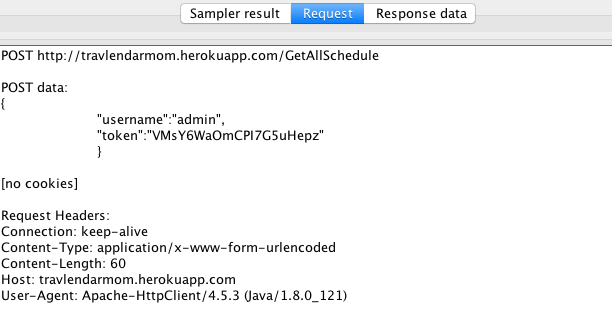
\includegraphics[width=0.8\textwidth]{Test/GetAllScheduleReq}
	\caption{The request sended to server for the GetAllSchedule servlet}
\end{figure}

\begin{figure}[H]
	\centering
	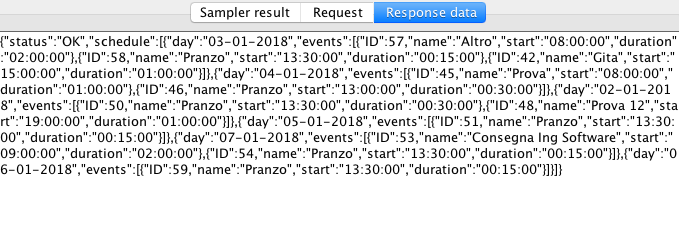
\includegraphics[width=0.8\textwidth]{Test/GetAllScheduleResp}
	\caption{The response of the server for the GetAllSchedule servlet}
\end{figure}


\begin{figure}[H]
	\centering
	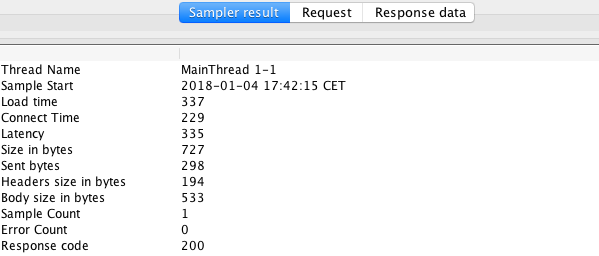
\includegraphics[width=0.8\textwidth]{Test/GetScheduleMain}
	\caption{The performance results (in millisecond) of the GetSchedule servlet on Heroku application server}
\end{figure}

\begin{figure}[H]
	\centering
	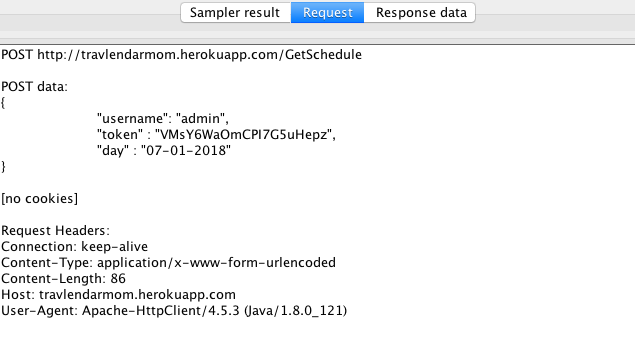
\includegraphics[width=0.8\textwidth]{Test/GetScheduleReq}
	\caption{The request sended to server for the GetSchedule servlet}
\end{figure}

\begin{figure}[H]
	\centering
	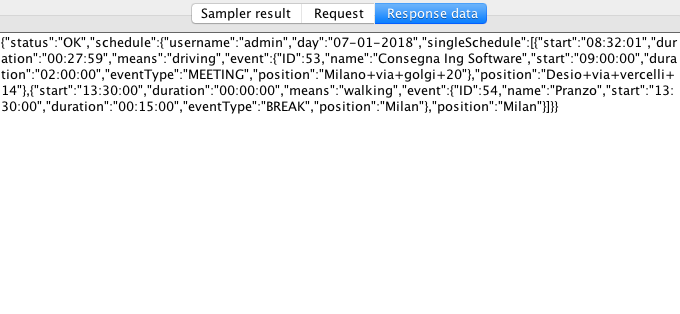
\includegraphics[width=0.8\textwidth]{Test/GetScheduleResp}
	\caption{The response of the server for the GetSchedule servlet}
\end{figure}

\section*{Client Testing}
With the aim to provide a test also at the client side of the application was created a purpose specific Python server to test the response of the client at some predetermined situation that the server provide statically. 
The test of the client will be provided in the source code in TestExtra/testClient folder and an example of the response is showed in the following pages. \\\newline
The Python server require to be executed with Python3 to support all its features, it also require two additional modules: Colorama and Flask those are available to download directly from command line by using python commands (that are different between the various OS).
In order to run the test in the same folder there are a "templates" folder which contains a specifically purposed client copy that must be at the same level of the Python server file (server.py).\\\newline
For all the endpoint there was a code that emulate the real server response, this allows to test the client side independently from the real application and web servers.
The server shows in the command line that run it the result of the different requests of the client and shows clearly, also using colors (red for errors and yellow for correct request), if the calls is successfull or not. \\\newline
In order to replicate the usage of the client testing server, the following command is required 
\begin{lstlisting}
# In TestExtra/testClient folder
python3 server.py
\end{lstlisting}
(Python 3 or later is required, please check on \textbf{https://www.python.org/}) for the download)
Then you have to access to your browser while the server is running and check the following address
\begin{lstlisting}
http://127.0.0.1:5000
\end{lstlisting}The following code show the example of the Login endpoint of the testing server.

\lstset{language=Python}
\begin{lstlisting}
	# Test del metodo del login
	@app.route('/Login', methods=['POST'])
	def login():
		if request.method == 'POST':
			data_loaded = json.loads((request.data).decode("utf-8"))
			if data_loaded['username'] == tempUsername and data_loaded['password'] == tempPassword:
				print(Fore.WHITE + Back.YELLOW + "### REQUEST made on /Login")
				pprint(data_loaded)
				print(Back.YELLOW + "==========")
				print(Fore.WHITE + Back.YELLOW + "### RESPONSE is:")
				my_response = {
					"status" : "OK",
					"token" : tempToken
				}
				pprint(my_response)
				print(Style.RESET_ALL)
				return json.dumps(my_response)
			else:
				print(Back.RED+ Fore.WHITE + "Error!!")
				pprint(data_loaded)
				my_response = {
					"status" : "KO",
					"token" : "Qualcosa e' andato male..."
				}
				pprint(my_response)
				return json.dumps(my_response)
\end{lstlisting}

In the following pictures will be showed a success and a fail of the request from the client.
\vspace{1cm}
\begin{figure}[H]
	\centering
	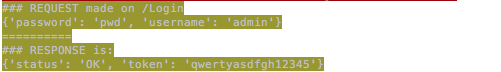
\includegraphics[width=1.1\textwidth]{Test/LoginSuccess}
	\caption{The correct request from the client}
\end{figure}
\vspace{1cm}
\begin{figure}[H]
	\centering
	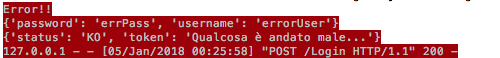
\includegraphics[width=1.1\textwidth]{Test/LoginError}
	\caption{The wrong request from the client}
\end{figure}


\chapter{Installation instructions}

To use the application you can proceed in to two different ways: you can access the site or you can install all the components in local. In the first case, you just have to access the url\\

\textbf{http://travlendarmom.herokuapp.com}.\\

Once the page is loaded, you have to log in clicking on "Get Started". After that, you can "Sign Up" or you can access directly using the test credentials
\begin{lstlisting}
	#Test credentials
	username = "admin"
	password = "pass"
\end{lstlisting}

In the second case, you have to download the following files:
\begin{itemize}
	\item JavaEE source files from the repository https://github.com/Gigioliva/OlivaMussiMoskwa
	\item Dump file for database Dump.sql in the same repository
	\item Eclipse for JavaEE http://www.eclipse.org/downloads/eclipse-packages/
	\item MySQL https://dev.mysql.com/downloads/mysql/
	\item MySQL Workbench https://dev.mysql.com/downloads/workbench/
	\item Tomcat 8.5.24 https://tomcat.apache.org/download-80.cgi
\end{itemize}
Once you have downloaded all the files, proceed with the MySQL installation wizard. As for the required parameters, please choose the following:
\begin{lstlisting}
	 port: "3306"
	 user:  "root"
	 password: "prova"
\end{lstlisting}

As the MySQL installation is completed, we suggest installing MySQL Workbench in order to manage the database using a GUI. \\
Now you have to carry out the dump of the data structure by CLI\\
(https://dev.mysql.com/doc/refman/5.7/en/mysqldump.html)
or by Workbench (Server $\,\to\,$ Data Import $\,\to\,$ Import from Self-Contained File $\,\to\,$ Dump Structure Only $\,\to\,$ Start Import).\\

Database initialization completed, install the server.

\begin{itemize}
	\item Unzip the Tomcat archive
	\item Open Eclipse and from "File" select "Import"
	\item Select "Existing Maven Projects", then the Travlendar folder downloaded from the repository (please be sure that a tick is present in side of the row of pom.xml)
	\item Once the project has been imported, click on it with the right mouse button and then press "Properties"
	\item Then select "Targeted Runtimes" and if there is no server, press "New ..." and follow the Tomcat configuration wizard
	\item Finally click on the project with the right button $\,\to\,$  Run As $\,\to\,$ Run On Server $\,\to\,$ select the server created $\,\to\,$ Finish
\end{itemize}

For any additional information about the installation of the whole system please write an email to: \textbf{gianluigi.oliva@mail.polimi.it} \\\newline

\section*{Additional notes}

\begin{itemize}
	\item The first request made to the web application can take some time to be performed. This is due to restrinctions imposed by Heroku.
	For more information about this please check the following link in scalability
	
	\textbf{https://devcenter.heroku.com/articles/dynos}
	
	\item After creating a new user, it is needed to add his preferences about Break Time and Means of Transport in order to add new Schedules and Events. If omitted this step, the application won't work correctly.
	
	\item In order to compile a new APK (if any change is needed), the following command is required
	\begin{lstlisting}
		phonegap build android
	\end{lstlisting}
	More information about Adobe PhoneGap can be founded at the following link: \textbf{https://phonegap.com}.
	
\end{itemize}


\chapter{Effort Spent}

While working on the project, we always met to discuss main topics to provide more consistence to the project:\\

\begin{tabular}{|p{0.2\textwidth}|p{0.8\textwidth}|}
	\hline
	\parbox[c][6ex]{6ex}{\centering \textbf{Name}} & \textbf{Effort}
	\\
	\hline
	\parbox[c][8ex]{6ex}{\centering Lukasz Moskwa} & Group 8h and 67h alone\\
	\hline
	\parbox[c][8ex]{6ex}{\centering Marco Mussi} & Group 8h and 62h alone\\
	\hline
	\parbox[c][8ex]{6ex}{\centering Gianluigi Oliva} & Group 8h and 65h alone \\
	\hline
\end{tabular}

\end{document}